\chapter{Appendix}
\label{appendixA}
\section{Grundriss Umsetzung}

   \begin{figure}[]
      \centering
      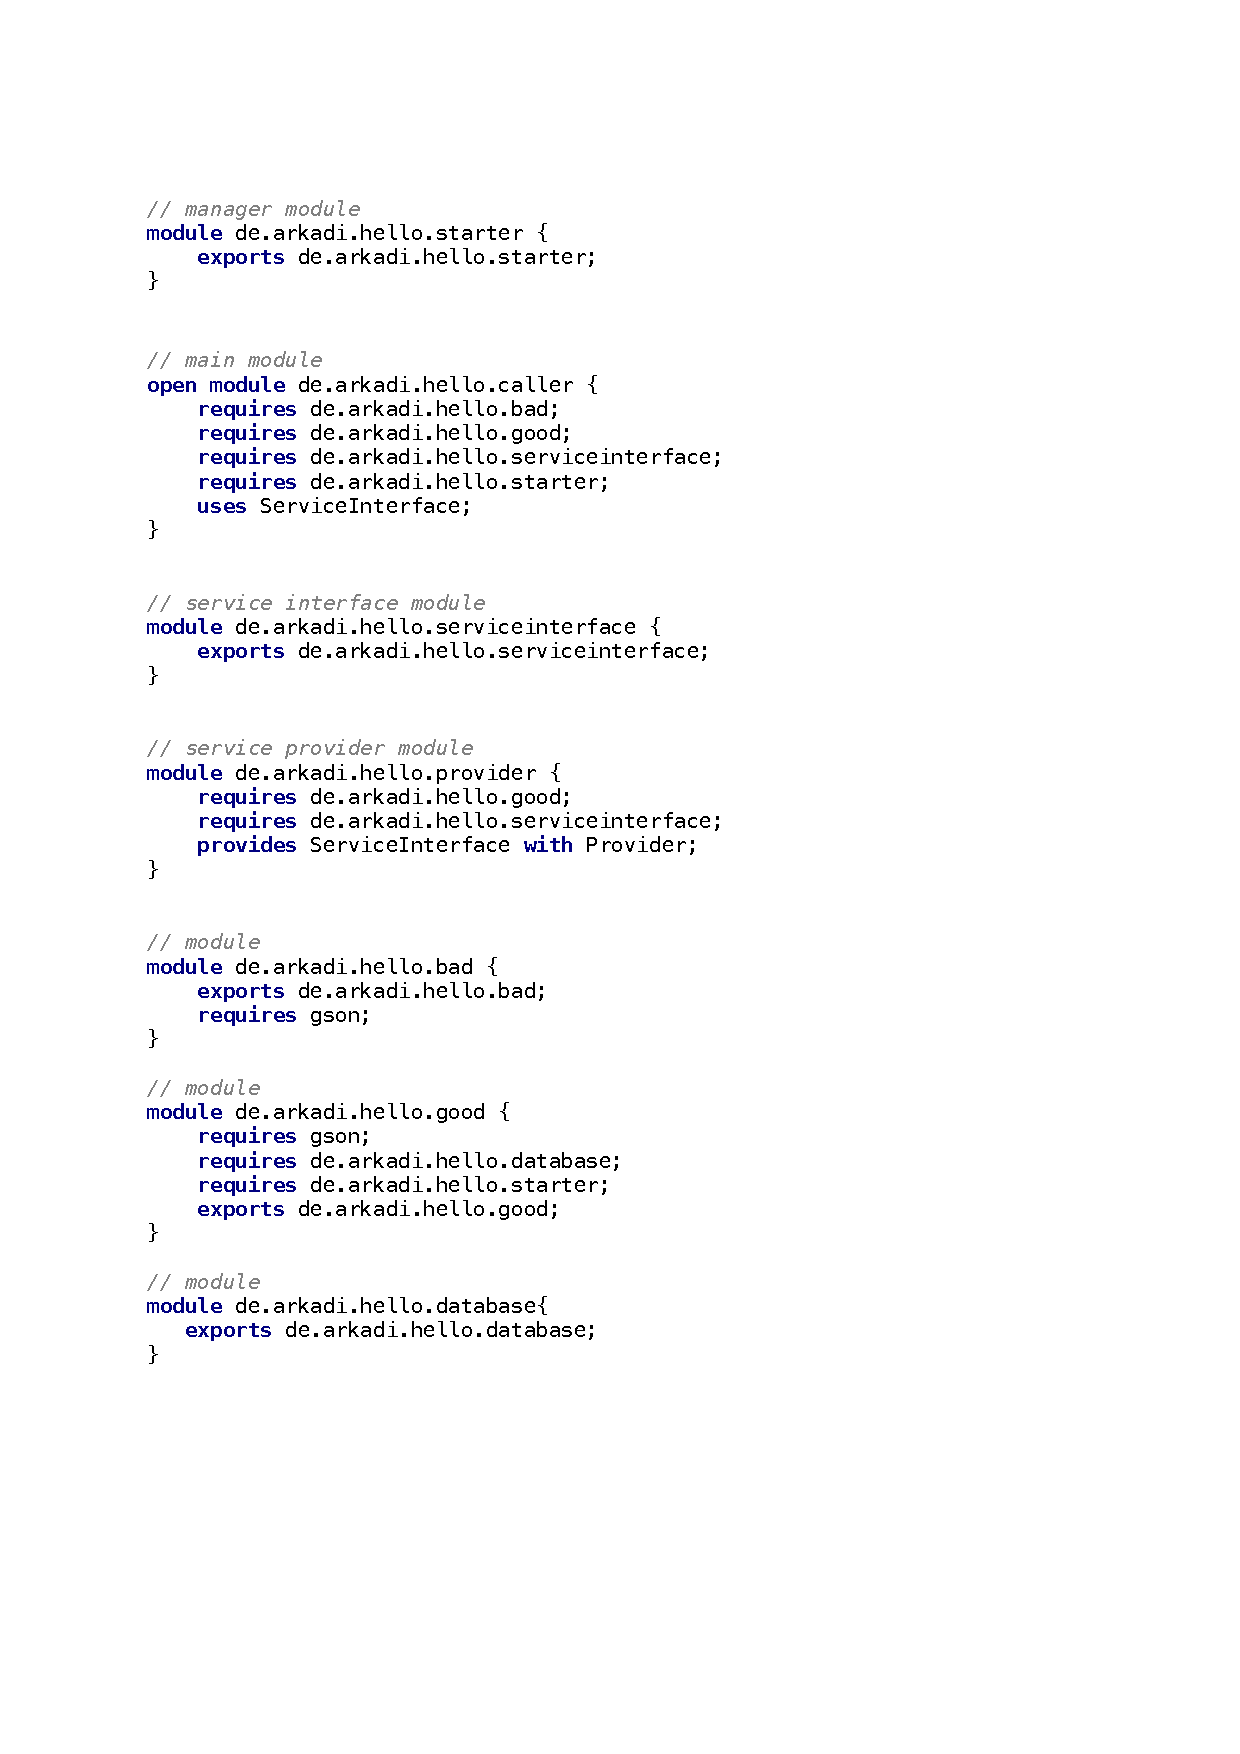
\includegraphics[]{material/images/appendix/modules.pdf}
      \caption{Grundriss Module}
      \label{fig:modulesG}
    \end{figure}

   \begin{figure}[]
      \centering
      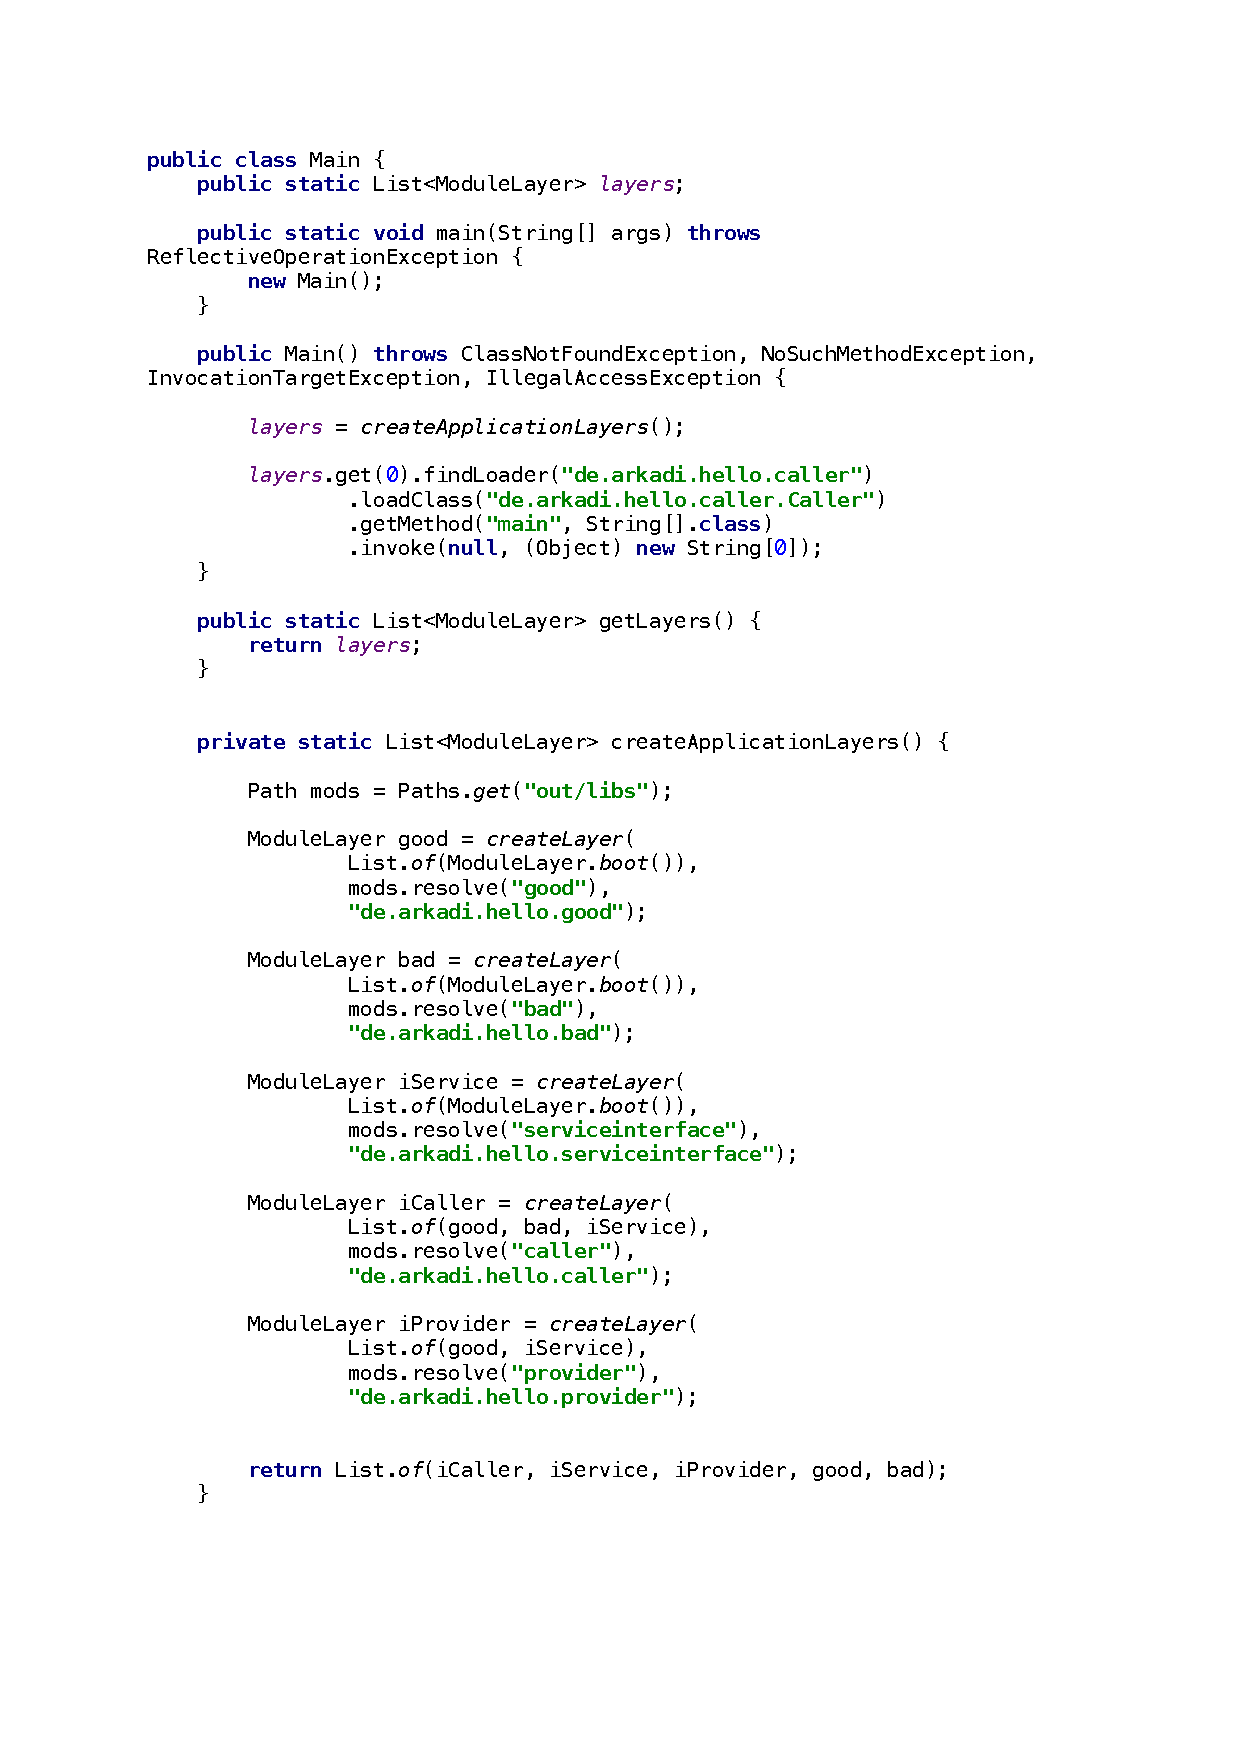
\includegraphics[scale=0.9]{material/images/appendix/mainA.pdf}
      \label{fig:starterA}
    \end{figure}

   \begin{figure}[]
      \centering
      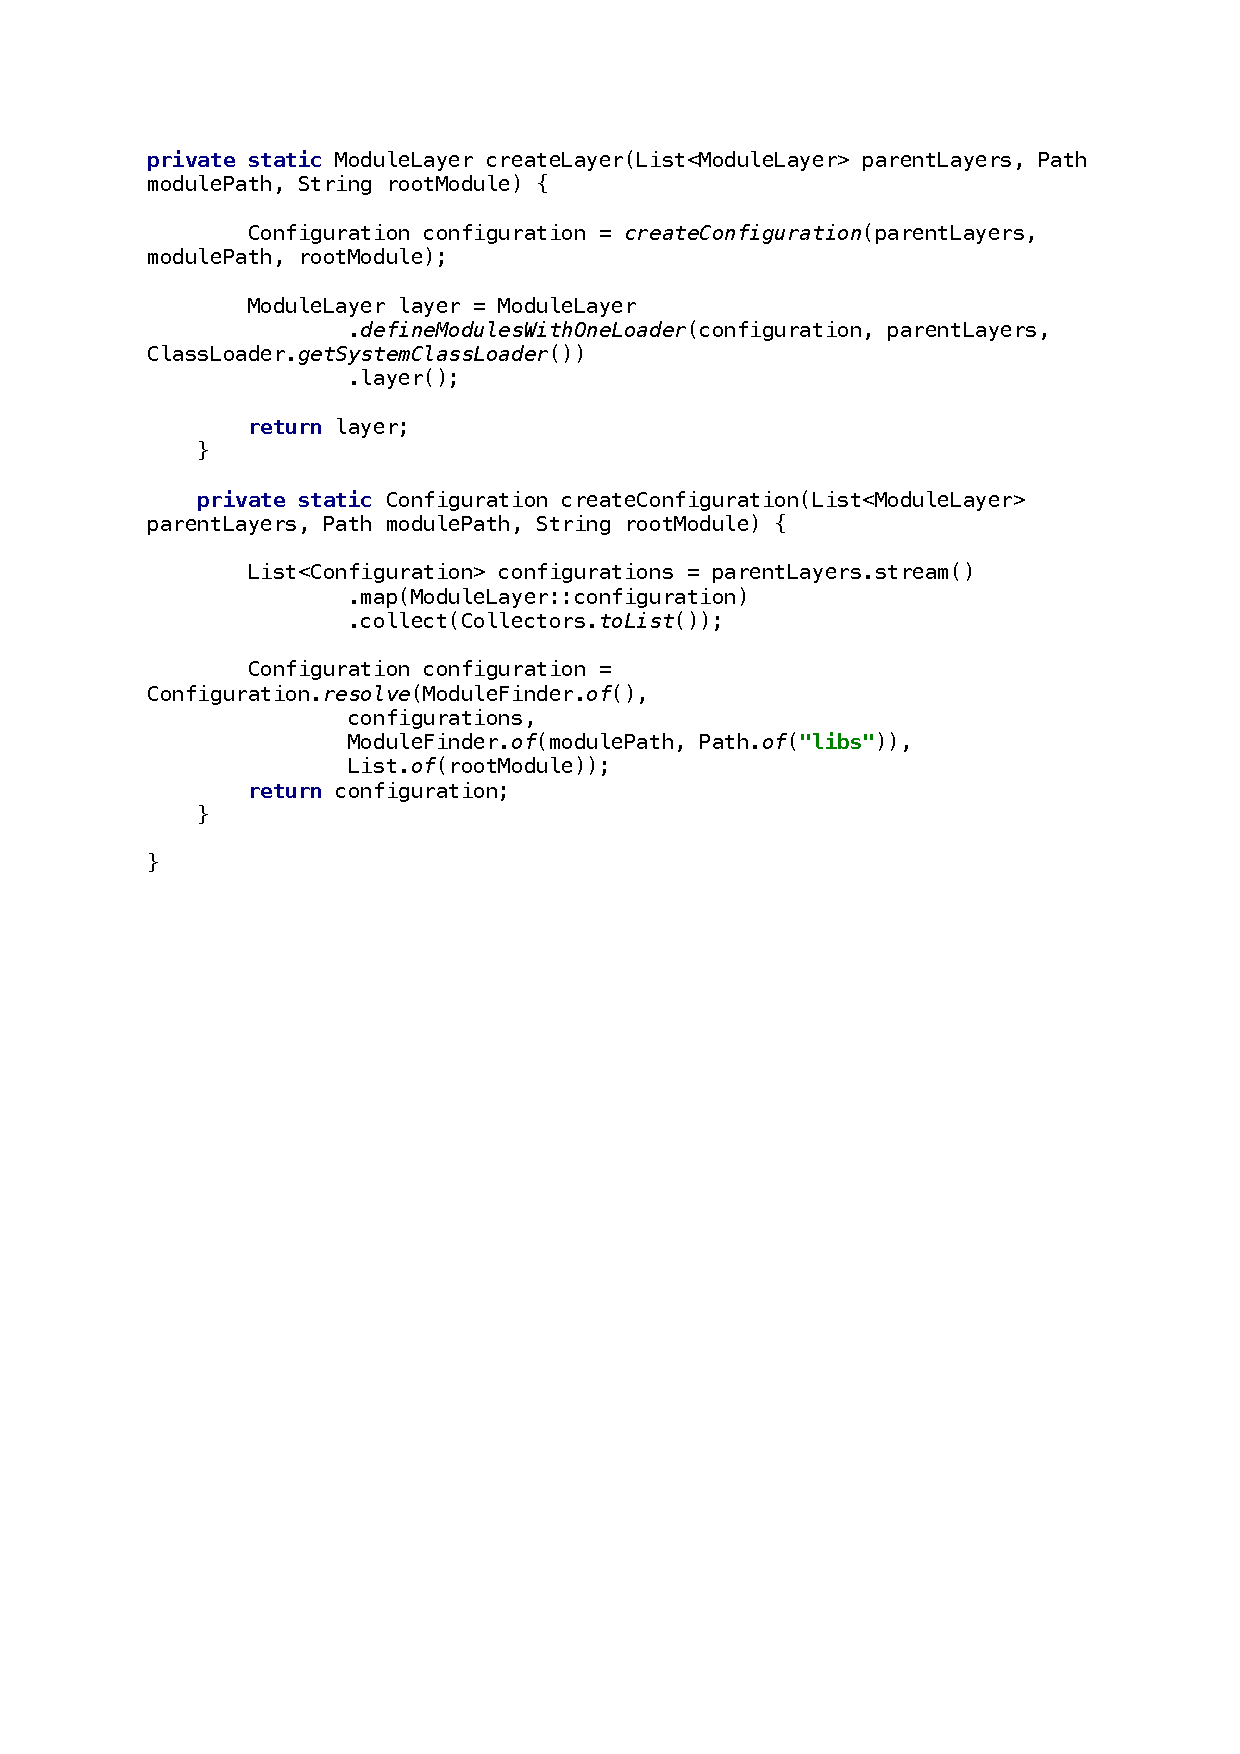
\includegraphics[width=\textwidth]{material/images/appendix/mainB.pdf}
      \caption{Starter Logik}
      \label{fig:starterB}
    \end{figure}